\documentclass[12pt, hyperref={bookmarks=false}, show notes]{beamer}
% Text
        \usepackage[T1]{fontenc}
        \usepackage[utf8]{inputenc}
        \usepackage[english]{babel}
        \usepackage[bitstream-charter]{mathdesign} % Serif font (Charter BT).
        \usepackage[scaled=0.84]{DejaVuSansMono} % Monospaced font.
        \def\sfdefault{SourceSansPro-TLF} % Sans serif font.
        \usepackage{textcomp}

% Maths
  \usepackage{amsmath}
  \usepackage{mathtools}
  \usepackage{siunitx}
  % Vector command
  \newcommand{\omatrix}[1]{\ensuremath{\boldsymbol{#1}}}

% Graphics
  \usepackage{graphicx}
  \usepackage[caption=false]{subfig}
        \usepackage{tikz}
  \usepackage{pgfplots}
  \pgfplotsset{compat=1.10}
        % ADD TIKZ LIBRARIES
  \usetikzlibrary{calc}
  \usetikzlibrary{arrows.meta}
  \usepackage{tikz-qtree}
  \usetikzlibrary{decorations.pathmorphing}
  \usetikzlibrary{matrix,shapes,positioning,fit}
  \usepgfplotslibrary{external}
  \tikzexternalize[prefix=graphics/tikz/]
  \tikzexternaldisable % Disable by default
  \usepackage{tabularx}
  \usepackage{pgfgantt}

        \usepackage{xcolor}
    \definecolor{color1}{cmyk}{100,50,0,0}   % blue
    \definecolor{color2}{cmyk}{0,80,100,0}   % vermillion
    \definecolor{color3}{cmyk}{97,0,75,0}    % blueish green
    \definecolor{color4}{RGB}{204,121,167}    % reddish purple
    \definecolor{color5}{RGB}{230,159,0}   % orange
   \usepackage{colortbl}
% Misc
\usepackage{booktabs}
\usepackage{enumerate}
\usepackage{pdfpages}
\usepackage{pgfpages}
\usepackage{setspace}
%\usepackage{multimedia}

\setbeamertemplate{navigation symbols}{}
\setbeamertemplate{caption}{\raggedright\insertcaption\par}
%\setbeamertemplate{bibliography item}[text]

%\usepackage{caption}
\usetheme{/amsterdam}
\date{October 11, 2016}

\usepackage{beamertheme/handoutWithNotes}
% Uncomment for handouts. Add \documentclass[12pt,handout]{beamer}
%\pgfpagesuselayout{4 on 1 with notes}[a4paper,border shrink=5mm]
% Comment for handouts.
\setbeameroption{show notes on second screen=right}

% Table of content dybde (0-index)
%\setcounter{tocdepth}{1}

% BibLaTeX
%\usepackage{csquotes}
%\usepackage[
%backend=bibtex,
%citestyle=numeric,
%bibstyle=numeric,
%maxcitenames=3,
%maxbibnames=99,
%url=true]{biblatex}
%\addbibresource{../rapport/references/refs.bib}
%\addbibresource{extrasources.bib}
%\usepackage{../style/biblatex_custom_formatting}

\graphicspath{{graphics/}{../../Report/graphics/}}

\begin{document}

%\captionsetup[figure]{font=small,singlelinecheck=off,justification=raggedright}

\title[Sentiment Knowledge Discovery in Twitter
Streaming Data]{TrashVision}
\author[\insertframenumber /\inserttotalframenumber]{SW703E15}

\begin{frame}
\Huge Learning Distributed Representations of Users
for Source Detection in Online Social Networks\\
\small The European Conference on Machine Learning and Principles and Practice of Knowledge Discovery in Databases 2016\\
\small Simon Bourigault, Sylvain Lamprier and Patrick Gallinari\\
\end{frame}

\begin{frame}
  \frametitle{Contents}
  \tableofcontents
  \note{
  \begin{itemize}
    \item Background
    \item Related Work
    \item Theory
    \item Evaluation
    \item Result
    \item Criticism
  \end{itemize}
}
\end{frame}

% PUT INPUTS HERE
\section{Introduction}

\begin{frame}
     \begin{center}
     	\huge Introduction
     \end{center}
\end{frame}

\begin{frame}
\frametitle{Problem of Role Detection in Online Social Networks}
Roles is network-specific and can not be used to in comparative analysis of other networks.


\note{
Explain social networks: \\
What is a social network\\
Why analyse them
}
\end{frame}

\begin{frame}
\frametitle{The Goal of the Article}
The purpose of this article, is to present a novel method that uses features based on interaction patterns and structural positions of a users to:
\begin{itemize}
\item Find persistent roles in dynamic data
\item Find roles that persists over time
\end{itemize}
This method should utilize the latent factors to identify the structure of the roles.

Persistent roles should occur in any social network

Based on the structure of the network
\note{
What is the article trying to do\\
Persistent roles consisting over time and datasets based on features.
}
\end{frame}






\section{Related Work}
\note{Not finished}
%Context
Dwork et al presented 4 Markov Chain methods. The fourth method, henceforth \MC had the most promising results, so it is the method we use for this paper.\cite{rank:aggregation}



\section{Methodology}

\begin{frame}
\begin{center}
     	\huge Methodology
     \end{center}
\end{frame}

\begin{frame}
\frametitle{The Approach}
\begin{figure}
\includegraphics[scale=0.14]{graphics/setup.pdf}
\end{figure}
\note{
feed the data\\
Snapshots:\\
Wanna se the roles lasting over time and networks.\\
Feature extraction:\\
Feature-based approach\\
For each snapshot\\
Role detection:\\
based on the features we wanne find the roles\\
Tracing roles:\\
Making sure the roles are persistent throughout the snapshots 
}
\end{frame}

\begin{frame}
\frametitle{The Data}
\begin{columns}
	\begin{column}{0.45\textwidth}
		Datasets:
			\begin{itemize}
				\item Facebook - Wall posts from one user to another
				\item Scratch - Comments on uploaded programming projects 
			\end{itemize}
		\end{column}
		\begin{column}{0.55\textwidth}
			\begin{figure}
				\includegraphics[scale=0.24]{graphics/directed_network.pdf}
			\end{figure}
		\end{column}
	\end{columns}
	\note{
	Facebook post and so one\\
	Scratch comments\\
	The networks are directed and timestamped.\\
	Edges are weighted based on the activity
	}
\end{frame}

\begin{frame}
\frametitle{Snapshots}
The datasets are split into a total of 26 snapshots:
\begin{itemize}
\item 7 from Facebook
\item 19 from Scratch
\end{itemize}
\begin{columns}
	\begin{column}{0.5\textwidth}
			\begin{block} {\small Social Network Graph}\centering
				$D = (N,E)$
			\end{block}
		\end{column}
		\begin{column}{0.5\textwidth}
			\begin{block} {\small Snapshot}\centering
				$S_t = (N_t,E_t)$
			\end{block}
		\end{column}
	\end{columns}
\note{
Non-overlapping\\
Snaps have same length defined as the observation windows $\Omega$\\
$\Omega$ is found by taking the average time between interacting nodes making sure 90\% of the is below $\Omega$
}
\end{frame}

\begin{frame}
\frametitle{Feature Selection}
\begin{columns}
	\begin{column}{0.35\textwidth}
		\begin{itemize}
			\item In-degree 
			\item Out-degree
			\item Weighted in-degree 
			\item Weighted out-degree
		\end{itemize}
	\end{column}
	
	\begin{column}{0.65\textwidth}
		\begin{figure}
			\includegraphics[scale=0.3]{graphics/directed_network.pdf}
		\end{figure}
	\end{column}
\end{columns}
\end{frame}
	
\begin{frame}
\frametitle{Feature Selection}
\textit{Reciprocity} is the rate a user is replayed.
\begin{columns}\centering
\begin{column}{0.5\textwidth}
	\begin{block}{\small Reciprocity}\centering
		$r = \frac{\text{Out-degree}^{<->}}{\text{Out-degree}}$
	\end{block}
\end{column}
\end{columns}
\begin{figure}
	\includegraphics[scale=0.32]{graphics/directed_network_example_reciprocity.pdf}
\end{figure}

\note{
L<-> is the edges going both ways\\
L is all outgoing edges
}
\end{frame}

\begin{frame}
\frametitle{Feature Selection}
The \textit{new activity count} feature is the number of new outgoing edges based on the difference of snapshot $S_t$ and $S_{t-1}$
\begin{columns}\centering
\begin{column}{0.5\textwidth}
	\begin{block}{\small New Activity Count}\centering
		$c = \text{Out-degree}_t - \text{Out-degree}_{t-1}$
	\end{block}
	\end{column}
\end{columns}

The feature \emph{social strategy} is the ratio of new outgoing edges over all outgoing edges 
\begin{columns}
\begin{column}{0.5\textwidth}
	\begin{block}{\small Social Strategy}\centering
		$s = \frac{\text{New Activity Count}}{\text{Out-degree}}$
	\end{block}
\end{column}
\end{columns}

\note{
L<-> is the edges going both ways\\
L is all outgoing edges
}
\end{frame}

\begin{frame}
\frametitle{Feature Selection}
The value of the feature \textit{betweenness centrality} is the product of the number of shortest paths passing through a vertex 
\begin{columns}\centering
\begin{column}{0.5\textwidth}
	\begin{block}{\small Betweenness Centrality}\centering
		$b(v) = \sum\limits_{s\neq v \neq t} \frac{\sigma_{st}(v)}{\sigma_{st}}$
	\end{block}
\end{column}\centering
\end{columns}
\begin{figure}
	\includegraphics[scale=0.32]{graphics/directed_network_example_betweenness.pdf}
\end{figure}

\note{
L<-> is the edges going both ways\\
L is all outgoing edges
}
\end{frame}

\begin{frame}
\frametitle{Feature Selection}
The feature \textit{PageRank} measures centrality based on ingoing edges and their influence
\begin{columns}
\begin{column}{0.8\textwidth}\centering
	\begin{block}{\small PageRank}\centering
		$pr(g) = 1-d + d(\frac{pr(b)}{2}+\frac{pr(e)}{4} + \frac{pr(f)}{1} + \frac{pr(i)}{4} + \frac{pr(j)}{1})$
	\end{block}
\end{column}
\end{columns}
\begin{figure}
	\includegraphics[scale=0.32]{graphics/directed_network_example_pagerank.pdf}
\end{figure}

\note{
L<-> is the edges going both ways\\
L is all outgoing edges
}
\end{frame}

\begin{frame}
\frametitle{Feature Selection}
\textit{Transitivity} measures is the local clustering coefficient which gives the probability of a vertexes neighbours being connected
\begin{columns}\centering
\begin{column}{0.8\textwidth}
	\begin{block}{\small Transitivity}\centering
		$C(v_i) = \frac{|\{e_{jk}\ :\  v_j,v_k\ \in\ N_i,\ e_{jk}\ \in\ E\}|}{k_i(k_i -1)}$
	\end{block}
\end{column}
\end{columns}
\begin{figure}
	\includegraphics[scale=0.32]{graphics/directed_network_example_transitivity.pdf}
\end{figure}

\note{
L<-> is the edges going both ways\\
L is all outgoing edges
}
\end{frame}


\begin{frame}
\frametitle{Selected Features}
Summary of the features
\begin{itemize}
\item In-degree
\item Out-degree
\item Weighted in-degree
\item Weighted out-degree
\item Reciprocity 
\item New activity count
\item Social strategy
\item Betweenness centrality
\item PageRang
\item Transitivity
\end{itemize}

Features omitted from the walk-though 
\begin{itemize}
\item Weighted PageRank
\item Weighted transitivity
\end{itemize}
\end{frame}

\begin{frame}
\frametitle{Feature Extraction}

The result of feature extraction is a features $\times$ users feature matrix

\begin{figure}
	\includegraphics[scale=.5]{matrix}
\end{figure}

The features in the matrix is normalized by the use of feature scaling so that all values is within the interval of 1 and 0

\note{
Next is feature extraction\\
The authors do not argue for the selected features\\
12 was selected.
}
\end{frame}

\begin{frame}
\frametitle{Role Discovery}
Roles are discovered by decomposing the feature matrix using NMF. This gives us:
\begin{itemize}
\item Basis matrix U, containing the feature characteristic for the roles
\item Coefficient matrix V, containing role membership weights for each user
\end{itemize}
\begin{columns}\centering
	\begin{column}{0.5\textwidth}
		\begin{block}{\small Non-negative Matrix Factorization}\centering
			$X \approx UV$
		\end{block}
		\end{column}
\end{columns}
\begin{figure}
\includegraphics[scale=.3]{graphics/nmf}
\end{figure}

\note{
\begin{itemize}
\item Frobenius NMF updated with euclidean distance
\item U and V are initialized with left and right matrix from nndsvd (Modified svd)

\end{itemize}
}
\end{frame}

\begin{frame}
\frametitle{Selection of L}
\begin{columns}
\begin{column}{0.5\textwidth}
\begin{block}{\small Root Mean Squired Error}\centering
$RMSE = \sqrt{\frac{1}{|X|} \sum\limits_{(u,f) \in X}(X_{u,f}-X'_{u,f})^2}$
\end{block}
\end{column}
\end{columns}
\begin{columns}
	\begin{column}{0.5\textwidth}
	\begin{figure}\caption{Facebook}
		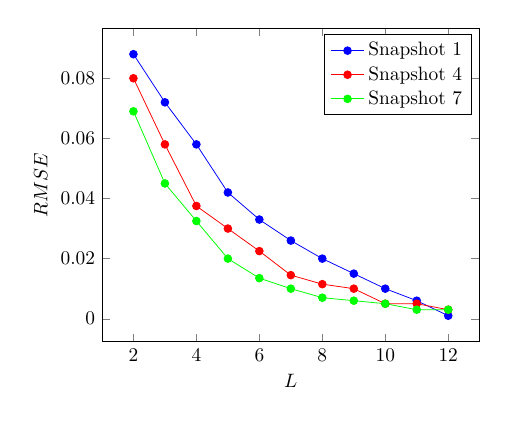
\begin{tikzpicture}[scale=0.7]
    \begin{axis}[
    	scaled ticks=false, 
    	tick label style={/pgf/number format/fixed},
        xlabel=$L$,
        ylabel=$RMSE$]
    \addplot[mark=*,blue] plot coordinates {
        (2, 0.088)
        (3, 0.072)
        (4, 0.058)
        (5, 0.042)
        (6, 0.033)
        (7, 0.026)
        (8, 0.020)
        (9, 0.015)
        (10, 0.010)
        (11, 0.006)
        (12, 0.001)
    };
    \addlegendentry{Snapshot 1}

    \addplot[color=red,mark=*]
        plot coordinates {
        (2, 0.08)
        (3, 0.058)
        (4, 0.0375)
        (5, 0.030)
        (6, 0.0225)
        (7, 0.0145)
        (8, 0.0115)
        (9, 0.01)
        (10, 0.005)
        (11, 0.005)
        (12, 0.003)
        };
    \addlegendentry{Snapshot 4}
    
    \addplot[color=green,mark=*]
        plot coordinates {
        (2, 0.069)
        (3, 0.045)
        (4, 0.0325)
        (5, 0.020)
        (6, 0.0135)
        (7, 0.010)
        (8, 0.007)
        (9, 0.006)
        (10, 0.005)
        (11, 0.003)
        (12, 0.003)
        };
    \addlegendentry{Snapshot 7}
    \end{axis}
\end{tikzpicture}	
\end{figure}
	\end{column}
	
	\begin{column}{0.5\textwidth}
	\begin{figure}\caption{Scratch}
		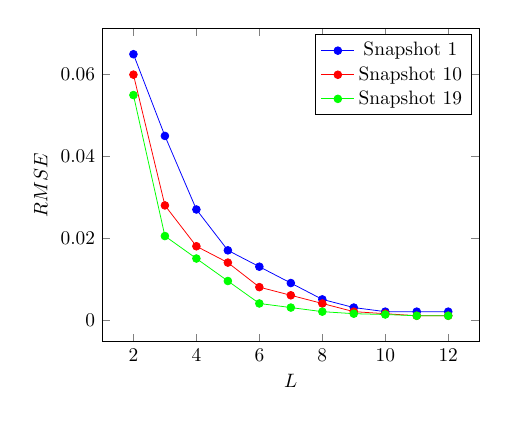
\begin{tikzpicture}[scale=0.7]
    \begin{axis}[
    	scaled ticks=false, 
    	tick label style={/pgf/number format/fixed},
        xlabel=$L$,
        ylabel=$RMSE$]
    \addplot[mark=*,blue] plot coordinates {
        (2, 0.065)
        (3, 0.045)
        (4, 0.027)
        (5, 0.017)
        (6, 0.013)
        (7, 0.009)
        (8, 0.005)
        (9, 0.003)
        (10, 0.002)
        (11, 0.002)
        (12, 0.002)
    };
    \addlegendentry{Snapshot 1}

    \addplot[color=red,mark=*]
        plot coordinates {
        (2, 0.06)
        (3, 0.028)
        (4, 0.018)
        (5, 0.014)
        (6, 0.008)
        (7, 0.006)
        (8, 0.004)
        (9, 0.002)
        (10, 0.0015)
        (11, 0.001)
        (12, 0.001)
    };
    \addlegendentry{Snapshot 10}
    
    \addplot[color=green,mark=*]
        plot coordinates {
        (2, 0.055)
        (3, 0.0205)
        (4, 0.015)
        (5, 0.0095)
        (6, 0.004)
        (7, 0.003)
        (8, 0.002)
        (9, 0.0015)
        (10, 0.0013)
        (11, 0.001)
        (12, 0.001)
        };
    \addlegendentry{Snapshot 19}
    \end{axis}
\end{tikzpicture}	
\end{figure}
	\end{column}
\end{columns}

\end{frame}

\begin{frame}
\frametitle{Tracing Roles}
\begin{columns}
\begin{column}{0.5\textwidth}
\begin{block}{\small Cosine Similarity}\centering
$sim(A_{i}, B_{i}) =\frac{\displaystyle\sum_{i=1}^n A_i B_i}{\sqrt{\displaystyle\sum_{i=1}^n A_{i}^2} \sqrt{\displaystyle\sum_{i=1}^n B_{i}^2}} $
\end{block}
\end{column}
\end{columns}

\begin{columns}
\begin{column}{0.5\textwidth}
Cosine similarity returns a value between -1 and 1
\begin{itemize}
\item -1 means that the vectors are opposites
\item 1 means they are exactly the same
\end{itemize} 
The article sets a threshold on 0.75 that roles from $S_t$ and $S_{t+1}$ must have similarity measure above
\end{column}
\begin{column}{0.25\textwidth}
\begin{figure}
\includegraphics[scale=.2]{role_matrix}
\caption{$U_t$}
\end{figure}
\end{column}
\begin{column}{0.25\textwidth}
\begin{figure}
\includegraphics[scale=.2]{role_matrix}
\caption{$U_{t+1}$}
\end{figure}
\end{column}

\end{columns}
\end{frame}
\section{Evaluation}\label{sec:evaluation}
In this section we show our evaluation of the aggregation methods described in Section \ref{sec:aggregations}.
\chapter{Setup} \label{structure}
\section{Pipeline}	\label{st:pipeline}
The group recommender is split into different stages, 

\begin{figure}
	\centering
	
\begin{tikzpicture}
	\fill circle (1.5);
	\end{tikzpicture}
	\caption{Efficiency evaluation of near-duplicate detection on the DS1 dataset \label{fig:neardup_performance}}
\end{figure}
\section{Results}

\begin{frame}
     \begin{center}
     	\huge Results 
     \end{center}
\end{frame}

\begin{frame}
	\frametitle{Methodology}
	The setup of the new test is the same as the previous tests
	\begin{itemize}
		\item The exact same random generated groups as in the previous tests
		\item Groups of the sizes 4, 8, 12, 16, 20, and 40
		\item There are 1000 groups of each size
		\item The preferences looked at is the top 10
	\end{itemize}
\end{frame}

\begin{frame}
\frametitle{Group Size 4}
\begin{figure}[h]
\centering
\begin{minipage}{.46\textwidth}\centering
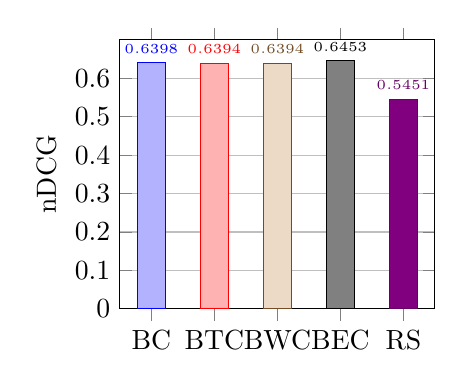
\begin{tikzpicture}
 \begin{axis}[
 	height=5cm,
 	width=4cm,
 	ybar =-10pt,
 	x = .8cm,
 	ymin=0.0, 
 	ymax=0.70,
 	ytick = {0, 0.1,0.2,0.3,...,0.70},
 	scaled y ticks = false,
	enlarge x limits ={abs=.4cm},
	nodes near coords,
    every node near coord/.append style={font=\tiny,/pgf/number format/.cd,precision=4},
 	ylabel={nDCG},
	xtick={0,1,2,3,4},  % NEW BIT
	xticklabels={BC, BTC, BWC, BEC, RS},
	%legend style={at={(0.5,-0.1)},
	%anchor=north,legend columns=-1},
	ymajorgrids = true,]

		\addplot coordinates {(0,0.6398)};    
		\addplot coordinates {(1,0.6394)};    
		\addplot coordinates {(2,0.6394)};    
		\addplot coordinates {(3,0.6453)};    
		\addplot coordinates {(4,0.5451)};
        %\legend{BC, BTC, BWC, BEC, Random}
     \end{axis}
\end{tikzpicture}
\end{minipage}
\begin{minipage}{.46\textwidth}\centering
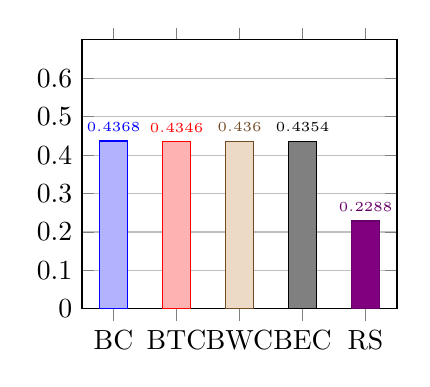
\begin{tikzpicture}
 \begin{axis}[
 	height=5cm,
 	ybar =-10pt,
 	x = .8cm,
 	ymin=0.0, 	
 	ymax=0.70,
 	ytick = {0,0.1,0.20,0.3,...,0.70},
	enlarge x limits ={abs=.4cm},
	nodes near coords,
    every node near coord/.append style={font=\tiny,/pgf/number format/.cd,precision=4},
	xtick={0,1,2,3,4},  % NEW BIT
	xticklabels={BC, BTC, BWC, BEC, RS},
	%legend style={at={(0.5,-0.1)},
	%anchor=north,legend columns=-1},
	ymajorgrids = true,]

		\addplot coordinates {(0,0.4368)};    
		\addplot coordinates {(1,0.4346)};    
		\addplot coordinates {(2,0.436)};    
		\addplot coordinates {(3,0.4354)};    
		\addplot coordinates {(4,0.2288)};
        %\legend{BC, BTC, BWC, BEC, Random}
     \end{axis}
\end{tikzpicture}
\end{minipage}
\end{figure}
\end{frame}

\begin{frame}
\frametitle{Group Size 12}
\begin{figure}[h]
\centering
\begin{minipage}{.46\textwidth}\centering
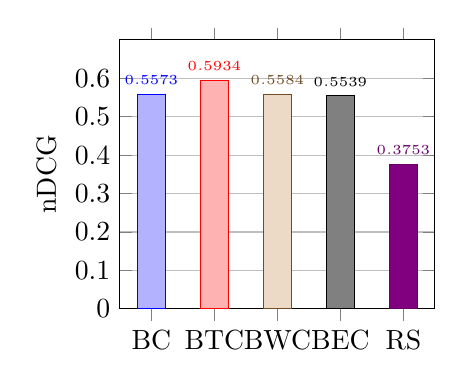
\begin{tikzpicture}
 \begin{axis}[
 	height=5cm,
 	width=4cm,
 	ybar =-10pt,
 	x = .8cm,
 	ymin=0.00, 
 	ymax=0.70,
 	ytick = {0,0.1,0.2,0.3,...,0.70},
 	scaled y ticks = false,
	enlarge x limits ={abs=.4cm},
	nodes near coords,
    every node near coord/.append style={font=\tiny,/pgf/number format/.cd,precision=4},
 	ylabel={nDCG},
	xtick={0,1,2,3,4},  % NEW BIT
	xticklabels={BC, BTC, BWC, BEC, RS},
	%legend style={at={(0.5,-0.1)},
	%anchor=north,legend columns=-1},
	ymajorgrids = true,]

		\addplot coordinates {(0,0.5573)};    
		\addplot coordinates {(1,0.5934)};    
		\addplot coordinates {(2,0.5584)};    
		\addplot coordinates {(3,0.5539)};    
		\addplot coordinates {(4,0.3753)};
        %\legend{BC, BTC, BWC, BEC, Random}
     \end{axis}
\end{tikzpicture}
\end{minipage}
\begin{minipage}{.46\textwidth}\centering
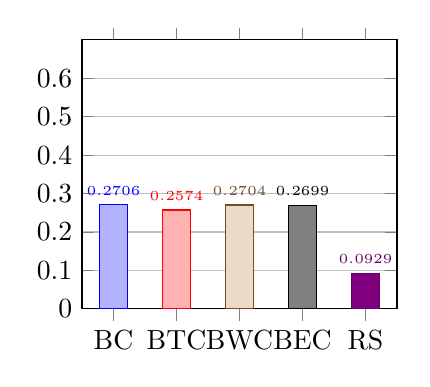
\begin{tikzpicture}
 \begin{axis}[
 	height=5cm,
 	ybar =-10pt,
 	x = .8cm,
 	ymin=0.0, 	
 	ymax=0.70,
 	ytick = {0,0.1,0.20,0.3,...,0.70},
	enlarge x limits ={abs=.4cm},
	nodes near coords,
    every node near coord/.append style={font=\tiny,/pgf/number format/.cd,precision=4},
	xtick={0,1,2,3,4},  % NEW BIT
	xticklabels={BC, BTC, BWC, BEC, RS},
	%legend style={at={(0.5,-0.1)},
	%anchor=north,legend columns=-1},
	ymajorgrids = true,]

		\addplot coordinates {(0,0.2706)};    
		\addplot coordinates {(1,0.2574)};    
		\addplot coordinates {(2,0.2704)};    
		\addplot coordinates {(3,0.2699)};    
		\addplot coordinates {(4,0.0929)};
        %\legend{BC, BTC, BWC, BEC, Random}
     \end{axis}
\end{tikzpicture}
\end{minipage}
\end{figure}
\end{frame}

\begin{frame}
\frametitle{Group Size 40}
\begin{figure}[h]
\centering
\begin{minipage}{.46\textwidth}\centering
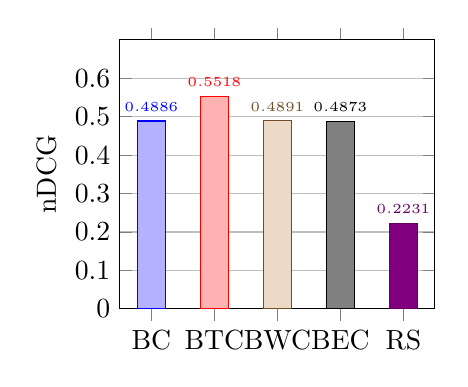
\begin{tikzpicture}
 \begin{axis}[
 	height=5cm,
 	width=4cm,
 	ybar =-10pt,
 	x = .8cm,
 	ymin=0.00, 
 	ymax=0.70,
 	ytick = {0,0.1,0.20,0.3,0.4,0.5,0.60},
 	scaled y ticks = false,
	enlarge x limits ={abs=.4cm},
	nodes near coords,
    every node near coord/.append style={font=\tiny,/pgf/number format/.cd,precision=4},
 	ylabel={nDCG},
	xtick={0,1,2,3,4},  % NEW BIT
	xticklabels={BC, BTC, BWC, BEC, RS},
	%legend style={at={(0.5,-0.1)},
	%anchor=north,legend columns=-1},
	ymajorgrids = true,]

		\addplot coordinates {(0,0.4886)};    
		\addplot coordinates {(1,0.5518)};    
		\addplot coordinates {(2,0.4891)};    
		\addplot coordinates {(3,0.4873)};    
		\addplot coordinates {(4,0.2231)};
        %\legend{BC, BTC, BWC, BEC, Random}
     \end{axis}
\end{tikzpicture}
\end{minipage}
\begin{minipage}{.46\textwidth}\centering
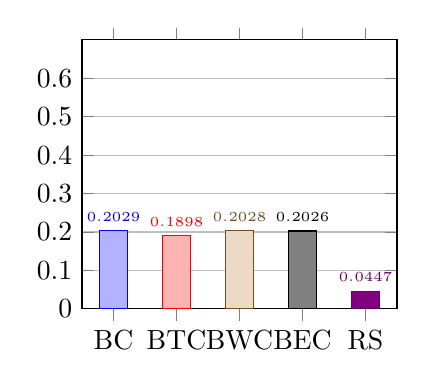
\begin{tikzpicture}
 \begin{axis}[
 	height=5cm,
 	ybar =-10pt,
 	x = .8cm,
 	ymin=0.0, 	
 	ymax=0.70,
 	ytick = {0,0.1,0.20,0.3,0.4,0.5,0.60},
	enlarge x limits ={abs=.4cm},
	nodes near coords,
    every node near coord/.append style={font=\tiny,/pgf/number format/.cd,precision=4},
	xtick={0,1,2,3,4},  % NEW BIT
	xticklabels={BC, BTC, BWC, BEC, RS},
	%legend style={at={(0.5,-0.1)},
	%anchor=north,legend columns=-1},
	ymajorgrids = true,]

		\addplot coordinates {(0,0.2029)};    
		\addplot coordinates {(1,0.1898)};    
		\addplot coordinates {(2,0.2028)};    
		\addplot coordinates {(3,0.2026)};    
		\addplot coordinates {(4,0.0447)};
        %\legend{BC, BTC, BWC, BEC, Random}
     \end{axis}
\end{tikzpicture}
\end{minipage}
\end{figure}
\end{frame}

\begin{frame}
	\frametitle{Possible Solutions}
	\begin{itemize}
		\item Calculate nDCG using the predicted ratings
		\item Ordering the individual ranked list by the average for the group
	\end{itemize}
\end{frame}

\begin{figure}[h]
\centering
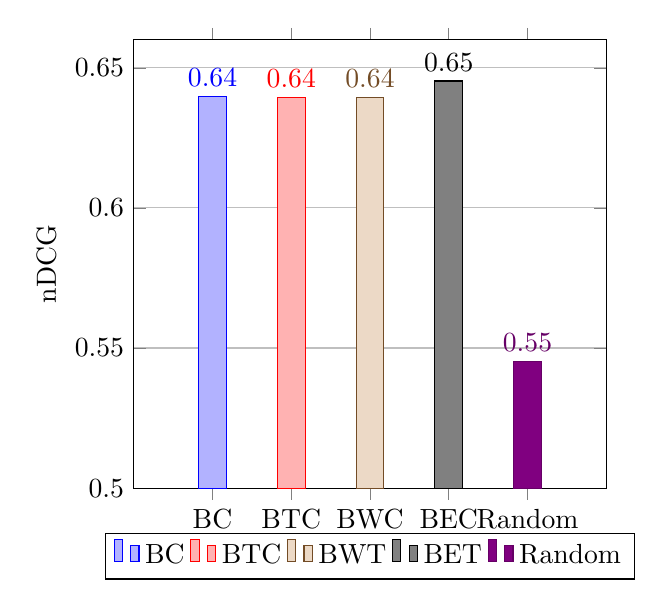
\begin{tikzpicture}
 \begin{axis}[
 	ybar =-10pt,
 	x = 1cm,
 	ymin=0.50, 
 	ymax=0.66,	
	enlarge x limits ={abs=1cm},
	nodes near coords,
 	ylabel={nDCG},
	xtick={0,1,2,3,4},  % NEW BIT
	xticklabels={BC, BTC, BWC, BEC, Random},
	legend style={at={(0.5,-0.1)},
	anchor=north,legend columns=-1},
	ymajorgrids = true,]

		\addplot coordinates {(0,0.6398)};    
		\addplot coordinates {(1,0.6393)};    
		\addplot coordinates {(2,0.6394)};    
		\addplot coordinates {(3,0.6453)};    
		\addplot coordinates {(4,0.5451)};
        \legend{BC, BTC, BWT, BET, Random}
     \end{axis}
\end{tikzpicture}
\caption{Group size 4}
\end{figure}

\begin{figure}[h]
\centering
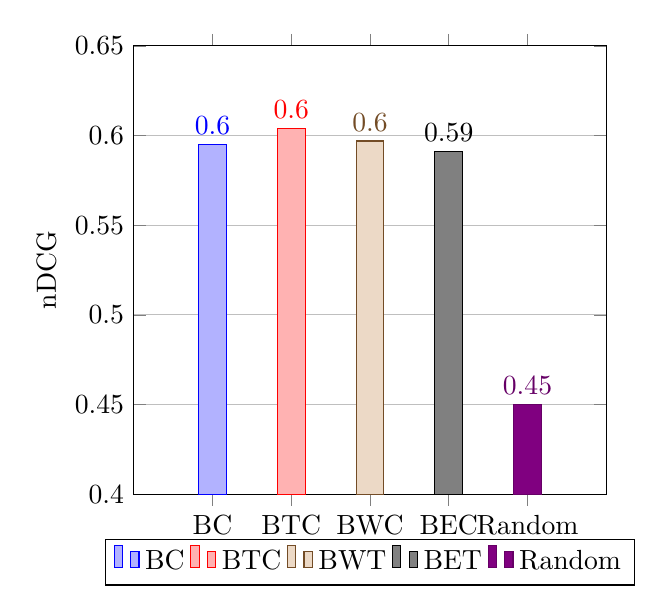
\begin{tikzpicture}
 \begin{axis}[
 	ybar =-10pt,
 	x = 1cm,
 	ymin=0.40, 	
 	ymax=0.65,
	enlarge x limits ={abs=1cm},
	nodes near coords,
 	ylabel={nDCG},
	xtick={0,1,2,3,4},  % NEW BIT
	xticklabels={BC, BTC, BWC, BEC, Random},
	legend style={at={(0.5,-0.1)},
	anchor=north,legend columns=-1},
	ymajorgrids = true,]

		\addplot coordinates {(0,0.5952)};    
		\addplot coordinates {(1,0.6040)};    
		\addplot coordinates {(2,0.5969)};    
		\addplot coordinates {(3,0.5910)};    
		\addplot coordinates {(4,0.4499)};
        \legend{BC, BTC, BWT, BET, Random}
     \end{axis}
\end{tikzpicture}
\caption{Group size 8}
\end{figure}

\begin{figure}[h]
\centering
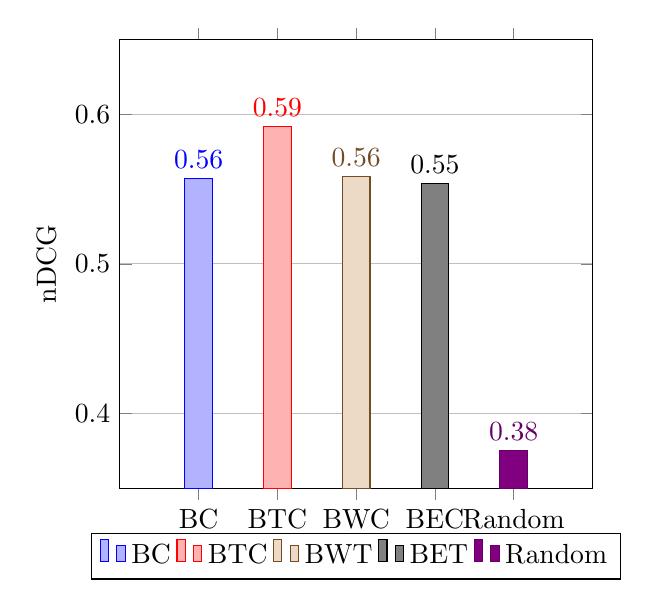
\begin{tikzpicture}
 \begin{axis}[
 	ybar =-10pt,
 	x = 1cm,
 	ymin=0.35, 	
 	ymax=0.65,
	enlarge x limits ={abs=1cm},
	nodes near coords,
 	ylabel={nDCG},
	xtick={0,1,2,3,4},  % NEW BIT
	xticklabels={BC, BTC, BWC, BEC, Random},
	legend style={at={(0.5,-0.1)},
	anchor=north,legend columns=-1},
	ymajorgrids = true,]

		\addplot coordinates {(0,0.5573)};    
		\addplot coordinates {(1,0.5922)};    
		\addplot coordinates {(2,0.5584)};    
		\addplot coordinates {(3,0.5539)};    
		\addplot coordinates {(4,0.3753)};
        \legend{BC, BTC, BWT, BET, Random}
     \end{axis}
\end{tikzpicture}
\caption{Group size 12}
\end{figure}

\begin{figure}[h]
\centering
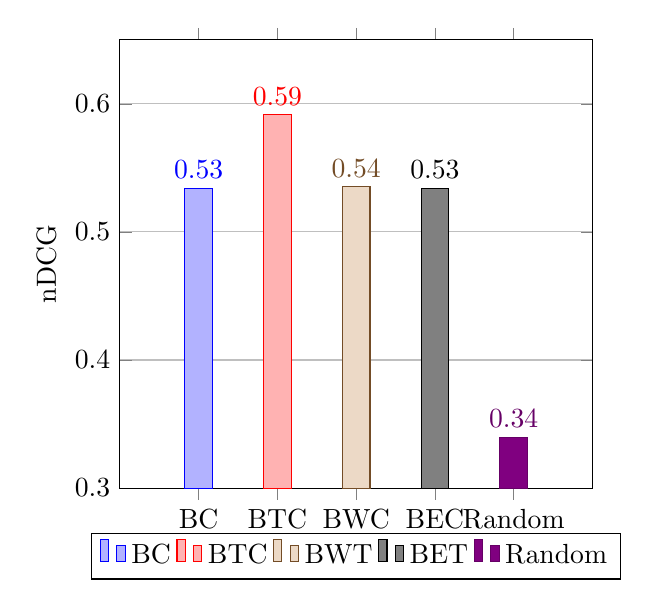
\begin{tikzpicture}
 \begin{axis}[
 	ybar =-10pt,
 	x = 1cm,
 	ymin=0.30, 	
 	ymax=0.65,
	enlarge x limits ={abs=1cm},
	nodes near coords,
 	ylabel={nDCG},
	xtick={0,1,2,3,4},  % NEW BIT
	xticklabels={BC, BTC, BWC, BEC, Random},
	legend style={at={(0.5,-0.1)},
	anchor=north,legend columns=-1},
	ymajorgrids = true,]

		\addplot coordinates {(0,0.5340)};    
		\addplot coordinates {(1,0.5913)};    
		\addplot coordinates {(2,0.5351)};    
		\addplot coordinates {(3,0.5340)};    
		\addplot coordinates {(4,0.3393)};
        \legend{BC, BTC, BWT, BET, Random}
     \end{axis}
\end{tikzpicture}
\caption{Group size 16}
\end{figure}

\begin{figure}[h]
\centering
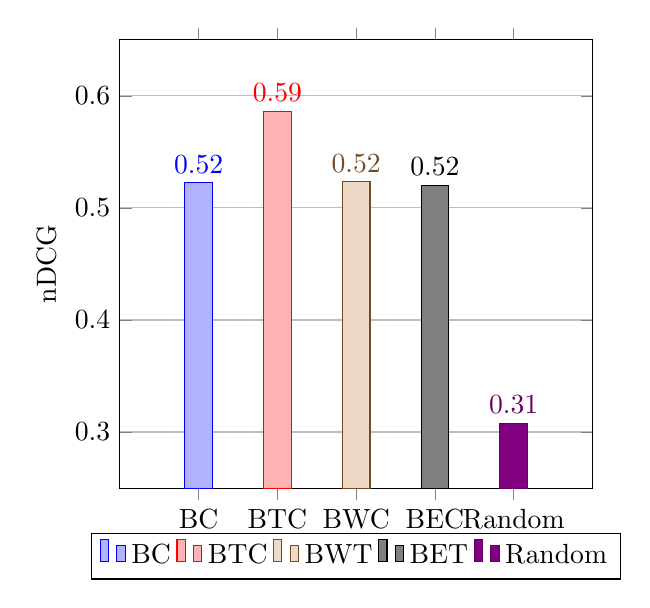
\begin{tikzpicture}
 \begin{axis}[
 	ybar =-10pt,
 	x = 1cm,
 	ymin=0.25, 	
 	ymax=0.65,
	enlarge x limits ={abs=1cm},
	nodes near coords,
 	ylabel={nDCG},
	xtick={0,1,2,3,4},  % NEW BIT
	xticklabels={BC, BTC, BWC, BEC, Random},
	legend style={at={(0.5,-0.1)},
	anchor=north,legend columns=-1},
	ymajorgrids = true,]

		\addplot coordinates {(0,0.5223)};    
		\addplot coordinates {(1,0.5862)};    
		\addplot coordinates {(2,0.5232)};    
		\addplot coordinates {(3,0.5199)};    
		\addplot coordinates {(4,0.3075)};
        \legend{BC, BTC, BWT, BET, Random}
     \end{axis}
\end{tikzpicture}
\caption{Group size 20}
\end{figure}

\begin{figure}[h]
\centering
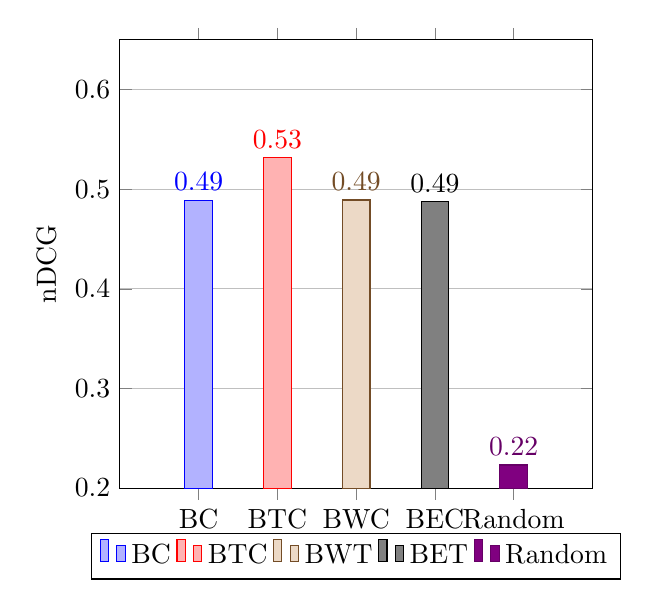
\begin{tikzpicture}
 \begin{axis}[
 	ybar =-10pt,
 	x = 1cm,
 	ymin=0.20, 
 	ymax=0.65,	
	enlarge x limits ={abs=1cm},
	nodes near coords,
 	ylabel={nDCG},
	xtick={0,1,2,3,4},  % NEW BIT
	xticklabels={BC, BTC, BWC, BEC, Random},
	legend style={at={(0.5,-0.1)},
	anchor=north,legend columns=-1},
	ymajorgrids = true,]

		\addplot coordinates {(0,0.4886)};    
		\addplot coordinates {(1,0.5314)};    
		\addplot coordinates {(2,0.4891)};    
		\addplot coordinates {(3,0.4873)};    
		\addplot coordinates {(4,0.2231)};
        \legend{BC, BTC, BWT, BET, Random}
     \end{axis}
\end{tikzpicture}
\caption{Group size 40}
\end{figure}
\section{Criticism}

\begin{frame}
        \centering
        \huge Criticism
\end{frame}

\begin{frame}
	\frametitle{Criticism}
	\begin{itemize}
		\item Inconsistent reference strategy. Did not always refer to their figures and formulas
		\item Latent Space
		\begin{itemize}
			\item Missing flow between concept and construction of representation model
			\item No reference to the picture
		\end{itemize}
		\item Size of dataset
		\item High concept, low technical
		\item Results of Content Integration for Twitter dataset
	\end{itemize}
\end{frame}

\section*{}

\end{document}
